\chapter{Telegestore}
\label{capitolo5}
\thispagestyle{empty}
In questo capitolo analizzeremo la realizzazione di un software pensato per inviare dei comandi alle centrali e alle periferiche che permettono la telegestione. In particolare in questo capitolo ci concentreremo sul software che gestisce  la comunicazione tra la centrale operativa e le diverse centrali sia come comunicazione diretta sia tramite l'utilizzo di ricevitori.\\
Nel capitolo successivo, invece, concentreremo la nostra analisi sul modulo che permette all'operatore di inviare i comandi al software che analizzeremo in questo capitolo.\\
In particolare questo software comunicherà con le centrali della marca \emph{Tecnoalarm} che permettono una connessione diretta per la telegestione tramite l'ausilio di un protocollo proprietario, il \emph{Tecno Out}. Inoltre, come accennato nel capitolo precedente, sfrutteremo il ricevitore AteArgo per inviare dei comandi anche alle periferiche Webu All-In-One.\\
Per quanto riguarda le funzionalità di questo software il suo scopo principale è quello di inviare comandi alle diverse periferiche, tuttavia per fornire maggiori informazioni all'operatore, ogni qualvolta che viene avviata la telegestione si richiedono alle periferiche ed alle centrali lo stato delle zone e delle partizioni in modo da avere sempre sotto controllo la situazione corrente.\\
\section{I protocolli di comunicazione}
Analizziamo ora come questo software comunicherà con le centrali, in particolare non ci addentreremo in dettaglio nei protocolli in quanto essi sono proprietari, ma analizzeremo la struttura del pacchetto e la comunicazione con la centrale o con il ricevitore interessato. In particolare analizzeremo i pacchetti di controllo del protocollo AteArgo per l'invio di comandi tra questo software e il corrispettivo ricevitore, e il protocollo \emph{Tecno Out} per la comunicazione con le centrali Tecnoalarm.
\subsection{Protocollo Tecno Out}
Il protocollo Tecno Out è un protocollo chiuso di proprietà di Tecnoalarm studiato per la comunicazione tra le centrali e sistemi di gestione remota come software di domotica o, come nel nostro caso, sistemi di telegestione.
\subsubsection{La struttura del pacchetto}
Pur non potendo addentrarci in particolare nella struttura del pacchetto analizzeremo alcuni punti salienti. Questo protocollo è orientato al byte e più in particolare il pacchetto ha una struttura molto semplice, il pacchetto è così costruito:
$$
\begin{array}{c}
\langle STX\rangle\langle codice\rangle\langle comando\rangle\langle len\rangle\langle dati\rangle\langle CRC16\rangle\\
\end{array}	 
$$
I diversi campi sono rispettivamente:
\begin{description}
	\item[STX:] campo composto da un unico byte e che delimita l'inizio del pacchetto;
	\item[codice:] questo campo è composto da 3 byte e contiene il codice utente per permettere l'accesso alla centrale
	\item[comando:] campo composta da un unico byte che identifica il comando da eseguire sulla centrale;
	\item[len:] indica la lunghezza del campo dati, essa varia in base al tipo di operazione da eseguire sulla centrale;
	\item[dati:] questo campo contiene le informazioni aggiuntive da utilizzare insieme al campo \emph{comando};
	\item[CRC16:] questo è il campo di controllo errori che sfrutta un algoritmo di CRC a 16 bit calcolato sul resto del pacchetto. Questo campo ha una lunghezza di due byte.
\end{description}
\subsubsection{La criptazione del pacchetto}
Questo protocollo sfrutta la criptazione AES a 128 bit. Ogni attore della comunicazione deve conoscere una chiave denominata \emph{PassPhrase} la quale verrà utilizzata insieme al vettore di inizializzazione.\\
Durante la prima fase il client invia un vettore di 17 byte contenete nei primi 16 byte il vettore di inizializzazione e nel diciassettesimo un valore predefinito criptato con il vettore appena inviato e con la PassPhrase. Il server quando riceve questo pacchetto salva i primi 16 byte come vettore e decripta il diciassettesimo con tale vettore e con la PassPhrase se il diciassettesimo byte decriptato corrisponde con il valore predefinito allora l'inizializzazione si conclude con successo e tutti i pacchetti successivi saranno criptati con tale vettore. In caso contrario il client chiude la connessione e riprova.\\
Non ci soffermeremmo oltre sulla criptazione in quanto nel codice questa operazione sarà effettuata da una libreria esterna e non implementata direttamente.
\subsubsection{La connessione}
La connessione è una semplice connessione client server tramite protocollo TCP/IP nel quale il nostro software svolge la funzione di client e la centrale d'allarme svolge quella di server. Questo significa che la centrale risponderà alle nostre richieste e non invierà messaggi se non interrogata. Durante la telegestione uno dei requisiti è quello di conoscere lo stato delle zone e delle partizioni perciò è necessario effettuare un polling per richiedere continuamente questi stati, ed all'inizio di ogni ciclo si controlla la presenza di nuovi comandi in coda.
In \fname{fig:contecno} vediamo come avviene la comunicazione, dopo la prima fase di inizializzazione del vettore di criptazione si prosegue con il ciclo di polling fino alla chiusura della connessione.
\begin{figure}
\centering
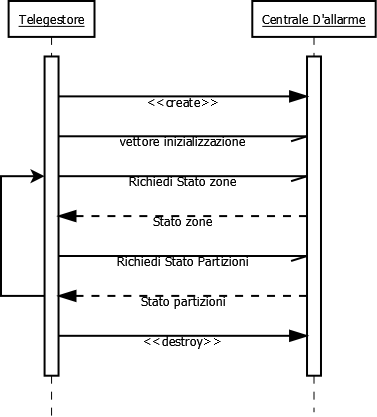
\includegraphics[width=0.7\linewidth]{pictures/contecno.png}
\caption{Scambio di messaggi tra software e centrali Tecnoalarm}\label{fig:contecno}	
\end{figure}
\subsubsection{I tipi di pacchetto}
In questo protocollo possiamo distinguere tre tipologie di pacchetto che sono:
\begin{itemize}
	\item messaggi di monitoring;
	\item messaggi di pilotaggio;
	\item messaggi di risposta.
\end{itemize}
I messaggi di monitoring servono per richiedere alla centrale di fornire informazioni riguardo al suo stato e a quello delle sue zone, i messaggi di pilotaggio sono quelli inviati dal nostro software verso la centrale per farle eseguire delle operazioni, infine, i messaggi di risposta sono quelli inviati dalla centrale per rispondere alle nostre richieste.
\paragraph{Messaggi di monitoring}
I messaggi di monitoring sono quei messaggi che il nostro software dovrà inviare alla centrale per richiedere lo stato di alcuni elementi, in particolare a noi interessa richiedere lo stato dei seguenti elementi:
\begin{itemize}
	\item lo stato delle zone;
	\item lo stato delle partizioni;
	\item lo stato della centrale;
	\item lo stato dei programmatori orari.
\end{itemize}
Per stato delle zone noi intendiamo se il singolo sensore è escluso, incluso oppure in allarme. Lo stato delle partizioni comporta sapere se esse sono inserite o disinserite o inserite solo in modo parziale. Per quanto riguarda le informazioni da conoscere sulla centrale, quelle che interessano a noi sono lo stato dell'alimentazione elettrica, quello della batteria e quello del tamper. Mentre l'unica informazione necessaria per i programmatori orari è se essi sono bloccati o in funzione.\\
Per reperire queste informazioni è necessario inviare alla centrale d'allarme il pacchetto formattato come precedentemente descritto con all'interno del campo codice un numero che ne identifica il comando. La centrale risponderà a questo comando inviando nel campo dati del pacchetto di risposta le informazioni. Prendendo come esempio le informazioni riguardanti la centrale noi inviamo il pacchetto specifico per richiedere queste informazioni e la centrale risponderà con un pacchetto con un unico byte nel campo dati. A questo byte deve essere applicata una maschera in AND per estrapolare le tre informazioni di cui necessitiamo.
\paragraph{Messaggi di pilotaggio}
I messaggi di pilotaggio servono per far eseguire delle azioni alla centrale d'allarme, per inviare i comandi da eseguire si utilizzano il pacchetto formattato così come indicato in precedenza con l'utilizzo di  opportuni codici. A differenza dei comandi di monitoraggio il campo dati questa volta contiene i valori da impostare sull'elemento selezionato. Ad esempio volendo escludere un opportuno sensore si invia alla centrale di allarme un pacchetto con l'opportuno valore nel campo comando e nei dati si inserisce il numero di zona e l'operazione da eseguire.\\
I comandi che interessano a noi sono solamente tre e riguardano le operazioni più comuni che gli operatori svolgono sulle centrali, ovvero, l'inclusione e l'esclusione di una zona, l'inserimento o il disinserimento di una partizione, ed infine il blocco o lo sblocco di un programmatore orario.
\paragraph{Messaggi di risposta}
I messaggi di risposta sono quelli che la centrale di allarme invia al nostro software essi possono essere di tre tipi:
\begin{itemize}
	\item ACK: in questo caso nel campo dati sono presenti eventuali risposte al messaggio inviato dal software come lo stato degli elementi richiesti.
	\item NACK: questo messaggio si riceve quando la centrale d'allarme non è in grado di interpretare il messaggio appena ricevuto e quindi non è in grado di dare una risposta.
	\item BUSY: questo tipo di messaggio di risposta si ottiene quando la centrale di allarme non è in grado di soddisfare le richieste perché occupata a svolgere altre operazioni o a soddisfare richieste precedenti.
\end{itemize}
L'ultimo messaggio è da tenere molto in considerazione in quanto esso limita il tempo di polling per gli stati della centrale, il protocollo infatti specifica che le richieste devono essere inviate con un intervallo minimo di 500ms.
\subsection{Protocollo Urmet}
Questo protocollo è lo stesso del capitolo precedente, in questo caso però analizzeremo i pacchetti necessari a richiedere lo stato degli ingressi e delle uscite e quello utilizzato per inviare i comandi, infine, analizzeremo le risposte a questi pacchetti.
\subsubsection{La struttura del pacchetto}
La struttura è quella che abbiamo visto nel capitolo precedente, si tratta di un protocollo basato su stringhe che formano una struttura XML con un tag di apertura seguito da una parte di header nella quali sono contenuti ora e data della trasmissione del pacchetto. Nel corpo del pacchetto invece troviamo le informazioni vere e proprie che dipendono dal tipo di pacchetto.
\subsubsection{La connessione}
Come si è visto la connessione con il software AteArgo è una connessione di tipo locale client-server nel quale il software di Urmet ricopre il ruolo di server. Tuttavia, pur essendo esso un server non permette la connessione di molteplici client questo ha comportato una problematica in quanto la connessione è necessaria al software ricevitore per mantenere la ricezione degli allarmi. Questo ci ha obbligati a pensare ad un meccanismo veloce e sicuro per far si che il ricevitore potesse inviare i comandi generati dal telegestore. Il meccanismo adottato è stato quello di una connessione socket tra \texttt{Ricevitore} e \texttt{Telegestore}, il \texttt{Telegestore} invia una stringa ad un server che viene eseguito ogni volta che viene avviato il software di ricezione. Questo meccanismo permette una comunicazione più rapida di quella che si avrebbe inserendo il comando in una tabella del database. 
Inoltre, questo tipo di comunicazione è stata pensata con un meccanismo di \emph{reques-replay} ed è quindi piuttosto affidabile.\\
Come nel caso precedente si attua un meccanismo di polling per richiedere lo stato degli ingressi e delle uscite di una determinata centrale, tuttavia in questo caso il polling no può essere molto stringente in quanto il software AteArgo effettua ogni volta la connessione con la periferica e non la mantiene aperta.
\subsubsection{I tipi di pacchetto}
Come abbiamo detto i tipi di pacchetto necessari per permettere di implementare le funzionalità richieste sono tre:
\begin{itemize}
	\item pacchetto di richiesta degli stati;
	\item pacchetto di comunicazione degli stati;
	\item pacchetto di comando.
\end{itemize}
\paragraph{Pacchetti di richiesta}
In questo tipo di pacchetto abbiamo che l'attributo del campo body è di tipo \emph{INO} nel campo body è presente solo l'identificativo della periferica di cui si vogliono conoscere gli stati.
\paragraph{Pacchetti di comunicazione degli stati}
In questo tipo di pacchetto abbiamo che l'attributo del campo body è uguale a quello della richiesta degli stati. In questo campo dopo le normali informazioni per identificare la periferica si ha una serie di campi per ogni ingresso od uscita che ne stabiliscono se è un contatto d'ingresso oppure un contatto d'uscita, se esso è impostato in modalità \emph{''normalmente aperto''} oppure in modalità \emph{''normalmente chiuso''} ed infine lo stato del contatto.
\paragraph{Pacchetto di comando}
In questo caso il pacchetto di comando contiene nella parte body le informazioni per identificare la centrale su cui effettuare i comandi e i contatti da attivare o disattivare.
\subsection{Protocollo Telegestore-Ricevitore}
Come abbiamo visto nella paragrafo precedente per permettere una comunicazione veloce ed efficiente tra il telegestore e il ricevitore che invia i comandi si è deciso di instaurare una connessione socket di tipo \emph{request-reply} tra i due software.\\
I due software si scambiano dei messaggi basati sullo stesso protocollo interno pensato per la comunicazione tra il server JBoss e il software di telegestione che vedremo nel capitolo successivo. Tuttavia qui accenniamo ad alcuni aspetti di questo pseudo-protocollo.\\
I pacchetti non sono altro che stringhe contenenti diversi campi separati da un carattere \emph{'';''}. I messaggi scambiati tra il telegestore e il software di ricezione hanno il seguente formato:
\begin{center}
	\textit{ce\_id;COM;elemento;numero;comando}
\end{center}
dove \texttt{ce\_id} è il codice che identifica la centrale, \texttt{elemento} indica su quale elemento eseguire il comando se esso è una zona o una partizione. Il campo \texttt{numero} indica il numero dell'elemento sul quale eseguire e, infine, il campo \emph{comando} contiene un codice per indicare quale azione eseguire sull'elemento identificato. Mentre il ricevitore, una volta eseguito il comando rimanda il pacchetto con indietro con l'aggiunta di un campo dopo comando con \emph{OK} se il comando è andato a buon fine o con \texttt{KO} se il comando è fallito.
\subsection{Altri protocolli}
Mentre scriviamo sono in implementazione nuovi protocolli di telegestione, alcuni simili o comunque riconducibili a quelli già analizzati come il \emph{CEI-ABI} protocollo standard per la ricezione di allarmi e la gestione di centrali d'allarme. La particolarità di questo protocollo è che mantiene sempre aperta la connessione con la centrale. Questa particolarità comporta un meccanismo tipo quello adottato con urmet per inviare i comandi in quanto è possibile aprire un'unica connessione ed è necessaria per la ricezione degli eventi.\\
Una seconda tipologia di telegestione in fase di sviluppo invece si basa sull'invio alle centrali di SMS preformatati e la centrale d'allarme risponde contattando la centrale operativa ed inviando le informazione richieste tramite i normali canali di comunicazione. Per questo tipo di comunicazione non è prevista la verifica dell'invio del comando e la comunicazione avviene tramite dei modem GPRS collegati su porte seriali.
\section{La struttura dati}
Come abbiamo visto in questo caso la comunicazione tra i diversi software avviene completamente tramite lo scambio di messaggi su socket. Tuttavia per poter tener traccia delle operazioni eseguite e dei comandi andati a buon fine si è deciso comunque di memorizzare sul database i comandi ed il loro stato in modo tale che in caso di crash del sistema sia possibile risalire agli eventi andati a buon fine e di quelli rimasti in sospeso.\\
La tabella realizzata a tale scopo è quella in \lname{lst:tabcodici}
\begin{lstlisting}[language=SQL,caption=Tabella comandi,label=lst:tabcodici]
CREATE TABLE comandi (
    cd_id integer NOT NULL DEFAULT nextval(('"comandi_cd_id_seq"'::text)::regclass),
    cd_tipo_comand integer,
    cd_tipo_element integer,
    cd_num_element integer,
    cd_stato character(1) DEFAULT 'n'::character varying,
    cd_risposta integer DEFAULT 0,
    cd_centrale character varying(5),
    cd_codice_hw character varying(30),
    CONSTRAINT cd_comandi_id_pkey PRIMARY KEY (cd_id)
)
\end{lstlisting}
dove i campi sono autoesplicativi, il campo stato indica se il comando è stato preso in gestione dal telegestore mentre il campo risposta indica la risposta che esso comunica al server JBoss. I campi \texttt{cd\_element} e \texttt{cd\_command} sono rispettivamente i campi associati ai valori che vengono trasmessi nel protocollo tra server in ascolto sul software \texttt{Ricevitore} e \texttt{Telegestore}.
\section{Architettura e realizzazione del sistema}
Analizziamo ora come è stato realizzato il sistema in particolare ci concentreremo su quella parte di software progettato per comunicare con le centrali d'allarme o con i ricevitori. Per quanto riguarda il funzionamento del software esso è molto semplice riceve una segnalazione da software JBoss e inizializza un thread che comunica con la centrale o con il ricevitore. Questo thread richiede più o meno periodicamente gli stati delle zone, delle partizioni e della centrale e li confronta con quelli precedenti nel caso in cui  vi sia una variazione tra lo stato precedente e quello attuale notifica al thread principale la variazione ed esso provvederà a notificarlo al software eseguito sul server JBoss.\\
Una precisazione è da fare per quanto riguarda la distinzione tra periferiche di backup e centrali d'allarme, le prime sono meno potenti ed hanno meno ingressi e non hanno la possibilità di dividerli in partizioni, tuttavia si comportano esattamente come delle centrali d'allarme; le seconde invece presentano un numero di uscite minore e solitamente sono adibite a funzioni specifiche come il collegamento con sirene esterne e quindi non sono controllabili come nel caso delle periferiche. Per uniformare il software si è deciso di trattare le periferiche di backup come fossero delle centrali d'allarme adottando però come convenzione il fatto che le partizioni nelle periferiche di backup rappresentano le uscite mentre le zone ne rappresentano gli ingressi. Questo meccanismo ci permetterà di attivare le uscite di una periferica semplicemente dando il comando di inserimento di una partizione. 
\begin{figure}[p]
	\centering
	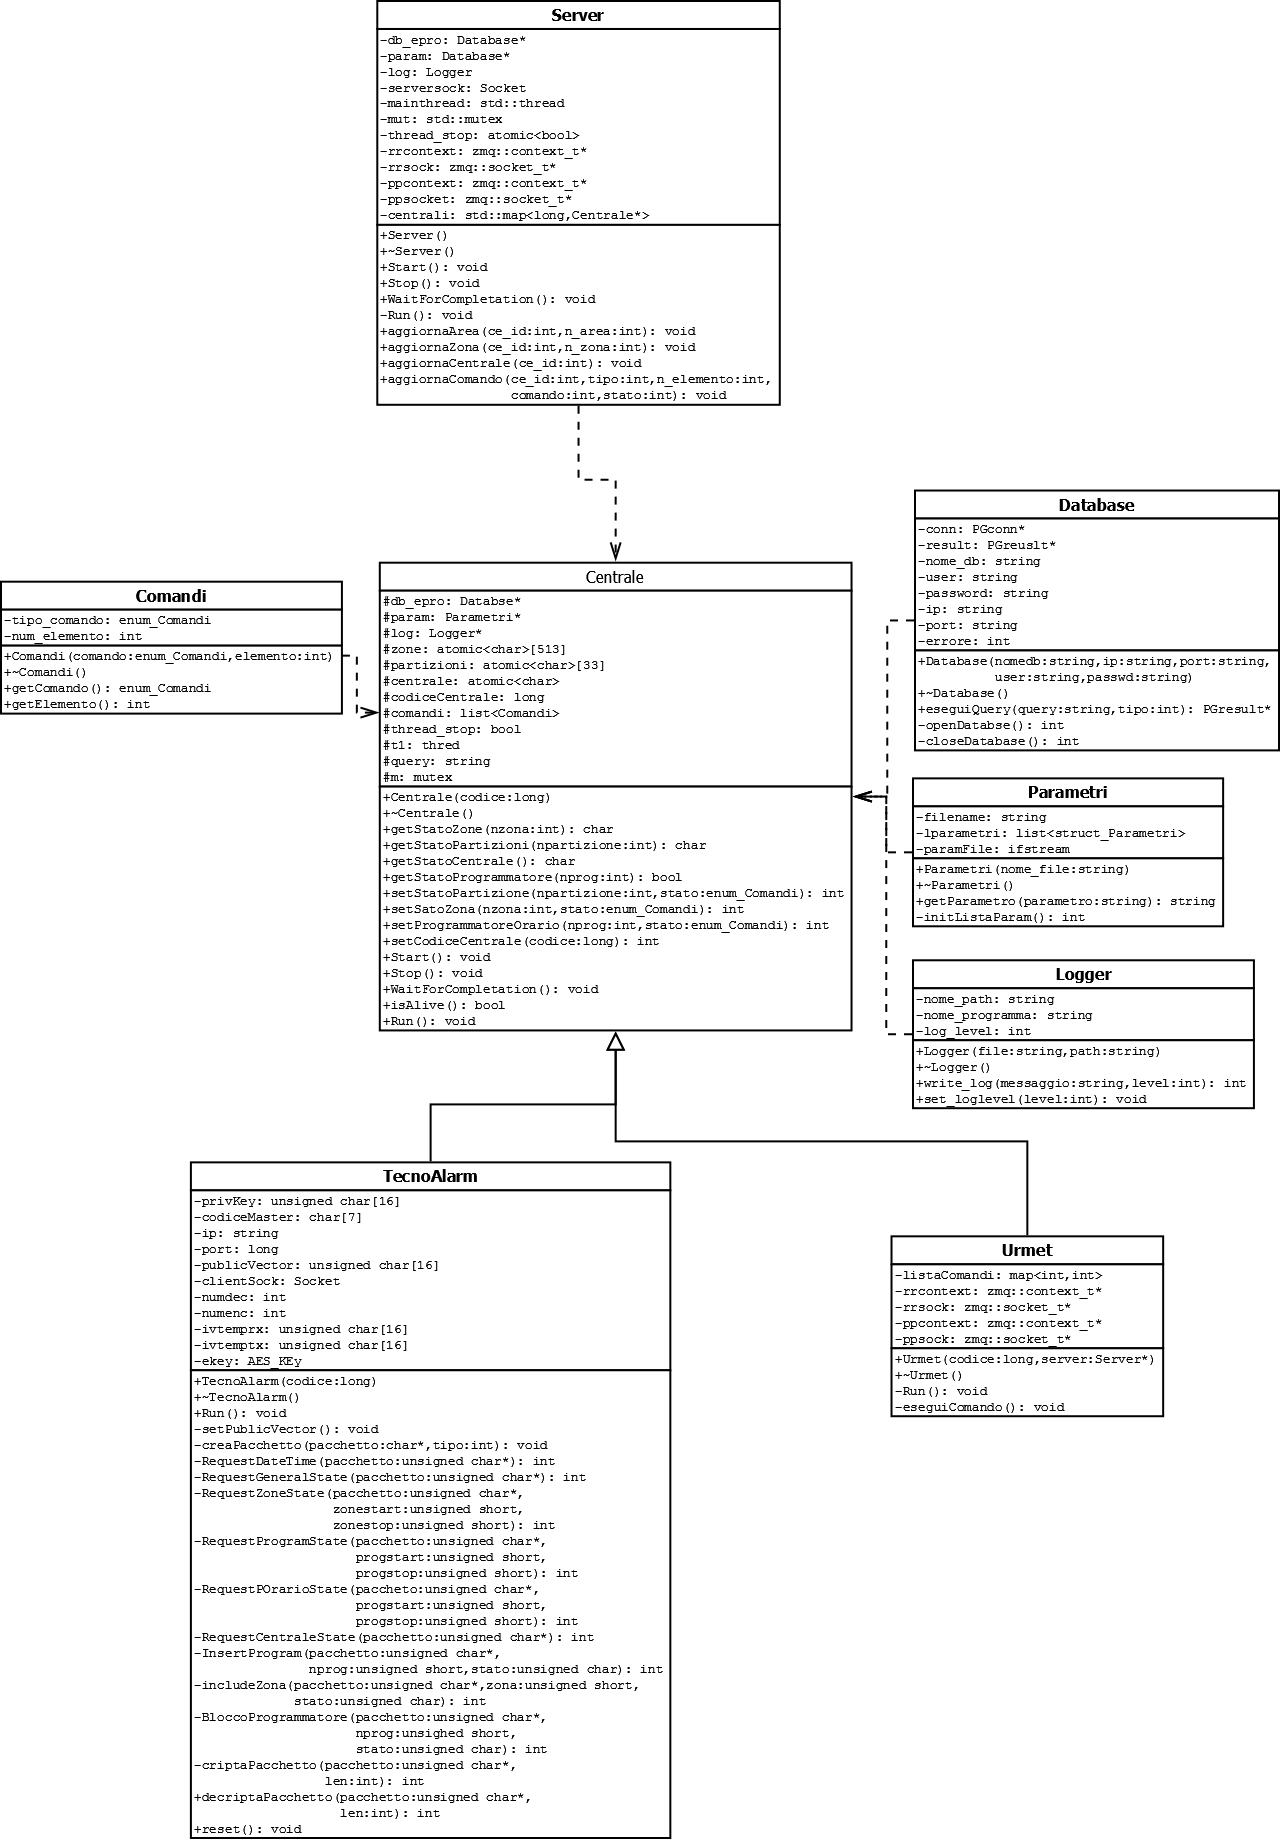
\includegraphics[width=\linewidth]{pictures/classitele.png}
	\caption{Schema delle classi del telegestore}\label{fig:classitele}
\end{figure}
\subsection{Le classi}
In \fname{fig:classitele} è mostrato lo schema delle classi del software. Analizziamo ora in dettaglio le diverse classi.
\subsubsection{Server}
Questa classe è la classe principale del software che gestisce la comunicazione con il software eseguito sul server JBoss. L'analisi di questa classe avverrà in maniera dettagliata nel prossimo capitolo.
\subsubsection{Centrale}
Questa classe è una classe astratta che serve da base per l'implementazione della telegestione delle diverse centrali di sicurezza. Essa prevede una serie di metodi per l'inserimento dei comandi in una \texttt{list<Comandi>} che poi sarà periodicamente controllata dal thread di esecuzione il quale preleverà il comando e lo eseguirà, questi metodi sono:
\begin{itemize}
\item \texttt{setStatoZona}
\item \texttt{setStatoPartizione}
\item \texttt{setStatoProgrammatoreOrario}
\end{itemize}
Oltre a questi metodi abbiamo una serie di metodi per prelevare l'ultimo stato memorizzato dei diversi elementi come lo stato delle zone, delle partizioni e della centrale, questi metodi sono:
\begin{itemize}
	\item \texttt{getStatoZona}
	\item \texttt{getStatoPartizione}
	\item \texttt{getStatoProgrammatoreOrario}
	\item \texttt{getStatoCentrale}
\end{itemize}
Essi restituiscono tutti come valore di ritorno un dato di tipo \texttt{char} dal quale si possono reperire tutte le informazioni riguardanti l'elemento richiesto semplicemente applicando una maschera in AND e valutando il valore dei singoli bit.\\
Il resto dei metodi servono per la gestione del thread principale, in particolare il metodo \texttt{Run()} è il metodo che deve essere implementato da tutte le classi che ereditano questa classe.
\subsubsection{Comandi}
Questa è una classe di supporto che memorizza il tipo di comando da eseguire e il numero dell'elemento sul quale eseguirlo.
\subsubsection{Tecnoalarm}
Questa classe implementa la telegestione per le centrali Tecnoalarm e ne implementa il protocollo. Essa estende la classe \texttt{Centrale} e ne implementa il metodo \texttt{Run}, questo metodo esegue il polling di richiesta degli stati richiedendo lo stato di tutte le zone e di tutte le partizioni e non solo di quelle attive; questo è possibile in quanto i tempi di comunicazioni sono molto ridotti. Quando viene rilevato un cambiamento rispetto ad uno stato precedente il thread utilizza l'attributo \texttt{Server} passato al costruttore per invocare i metodi \texttt{aggiornaArea}, \texttt{aggiornaZona} e \texttt{aggiornaPartizione} i quali creano ed inviano un messaggio ai moduli in esecuzione sul JBoss. Ad ogni ciclo, inoltre, il thread controlla che la lista dei comandi sia vuota, in caso non lo fosse preleva il primo comando della lista ed invia il comando alla centrale telegestita.\\
Gli altri metodi sono a supporto del metodo \texttt{Run} in particolare tutti i metodi esclusi \texttt{criptaPacchetto}, \texttt{decriptaPacchetto} e \texttt{reset} non fanno altro che riempire un array di caratteri con i valori necessari per creare un pacchetto valido secondo lo standard del protocollo, in particolare il metodo \texttt{creaPacchetto} riempie i campi comuni come il byte di start o il codice utente, gli altri metodi riempiono il campo dati e il campo codice in base ai valori passati dai parametri ed al tipo di metodo invocato. Il metodo \texttt{criptaPacchetto} serve per criptare il pacchetto prima dell'invio mentre il metodo \texttt{decriptaPacchetto} esegue l'operazione di decriptazione all'arrivo di un nuovo messaggio. Il metodo \texttt{reset} viene invocato nel caso in cui vi siano problemi di connessione o di decodifica dei messaggi, esso chiude la connessione resetta i valori di criptazione e reinizializza la connessione.
\subsubsection{Urmet}
Questa classe implementa la logica per la telegestione delle periferiche Urmet. Essa estende la classe \texttt{Centrale} e ne implementa il metodo \texttt{Run}; questo metodo in realtà non implementa il vero e proprio protocollo, esso invia tramite socket un messaggio al software \texttt{Ricevitore} ed in particolare alla classe che implementa il protocollo AteArgo. In questo messaggio sono contenute tutte le informazioni necessarie per creare un pacchetto di comando al ricevitore AteArgo ed il software ricevitore risponde alle richieste tramite lo stesso socket.
Il funzionamento è simile a quello della classe TecnoAlarm, ovvero dopo la creazione il software richiede periodicamente gli stati della periferica e li confronta con quelli salvati in precedenza nel caso di variazione il thread, tramite l'istanza di \texttt{Server} passata nel costruttore notifica il cambiamento al server principale.
\subsubsection{Parametri}
Questa classe è stata pensata per supportare l'esecuzione del programma, in particolare essa si occupa di aprire e leggere da un file i parametri necessari per l'esecuzione del programma come ad esempio l'indirizzo IP del database, il nome utente necessario per la connessione, o ancora i parametri di connessione dei vari ricevitori. In particolare il metodo \texttt{initListaParametri} apre il file legge i diversi parametri suddivisi per riga e li carica in una lista chiamata \texttt{lparametri} la quale è una struttura che contiene il nome del parametro ed il suo valore.\\
Tramite il metodo \texttt{getParametro} le altre classi possono recuperare il valore assegnato ad un determinato parametro.
\subsubsection{Database}
Questa è un'altra casse di supporto che gestisce la connessione e le interrogazioni al database, in particolare il metodo \texttt{eseguiQuery} riceve in ingresso una stringa che contiene la query da eseguire ed un campo integer che indica se la query si aspetta un risultato oppure no. Questo meccanismo ci permette di eseguire la query in modo tale da non dover analizzare il risultato in caso di inserimenti del database.
\subsubsection{Logger}
Questa è l'ultima classe di supporto e fornisce gli strumenti per eseguire un sistema di log anche con diversi livelli di notifica. In particolare, istanziando un nuovo logger per istanze diverse di classi è possibile specificare per ogni istanza quale sia il livello di log da mantenere e quale nome associare al messaggio di log.
\subsection{Implementazione}
Anche questo software è stato sviluppato in linguaggio C++ aggiornato allo standard del 2011 (ISO/IEC 14882:2011\cite{c++11}) il quale supporta meglio il multi-threading e per fare ciò si è deciso di utilizzare il compilatore gcc-4.8 l'ultimo rilasciato al momento dell'implementazione. I vantaggi sono la possibilità di utilizzare i thread nativi del linguaggio e anche i tipi \emph{atomici} non presenti nelle versioni precedenti.\\
Per la comunicazione tra la classe \texttt{Server} e il software eseguito nel JBoss e tra la classe \texttt{Urmet} e il software \texttt{Ricevitore} è stato utilizzato il framework \emph{ZeroMQ}\cite{zmq} aggiornato alla versione 1.3 questo framework permette la creazione di diversi patern di comunicazione come il \emph{request-replay} o il \emph{public-subscribe} senza dover preoccuparsi di gestire la connessione o di controllare il corretto invio e ricezione dei messaggi.
\subsubsection{Centrale}
La classe centrale è una classe astratta in quanto al suo interno presenta il metodo virtuale \texttt{Run} dichiarato come segue:
\begin{lstlisting}[language=C++,caption=Metodo astratto Run]
virtual void Run ()=0;
\end{lstlisting}
Per quanto riguarda i metodi \texttt{getStato\emph{XXX}} essi non  fanno altro che restituire il valore del parametro corrispondente, un esempio è il metodo \texttt{getStatoZone} mostrato nel \lname{lst:getzone}. Esso non fa altro che restituire il valore richiesto, i problemi di concorrenza sui dati sono evitati in quanto le operazioni che vengono eseguite sono sempre atomiche in quanto i dati sono dichiarati \texttt{atomic}
\begin{lstlisting}[language=C++,caption=Metodo getStatoZone,label=lst:getzone]
char Centrale::getStatoZone(int nzona) {
    return zone[nzona];
}
\end{lstlisting}
I metodi \texttt{setStato\emph{XXX}} invece non fanno altro che aggiungere un'istanza di \texttt{Comando} alla lista comandi, un esempio è il metodo \texttt{setStatoPartizioni} mostrato nel \lname{lst:setpart}.
\begin{lstlisting}[language=C++,caption=Metodo setStatoPartizioni,label=lst:setpart]
int Centrale::setStatoPartizione(int npartizione, enum_Comandi stato) {
    Comandi nuovo(stato,npartizione);
    comandi.push_back(nuovo);
    return 1;
}
\end{lstlisting}
Il resto dei metodi è utilizzato per gestire il thread \texttt{Run}.
\subsubsection{Tecnoalarm}
Questa classe implementa il protocollo \emph{TecnoOut} in particolare il metodo \texttt{Run} implementa il polling e richiede periodicamente gli stati di zone partizioni e centrale, ad ogni ciclo inoltre verifica la lista dei comandi ed in caso essa non sia vuota invia il comando alla centrale.\\
In \fname{fig:flussotecno} viene mostrato il diagramma di flusso delle operazioni che esegue il metodo \texttt{Run}. Ad ogni richiesta degli stati il metodo confronta gli stati ricevuti con quelli precedenti e nel caso vi siano variazioni sfruttano l'istanza di \texttt{Server} per comunicarlo al livello più alto del software.
\begin{figure}
	\centering
	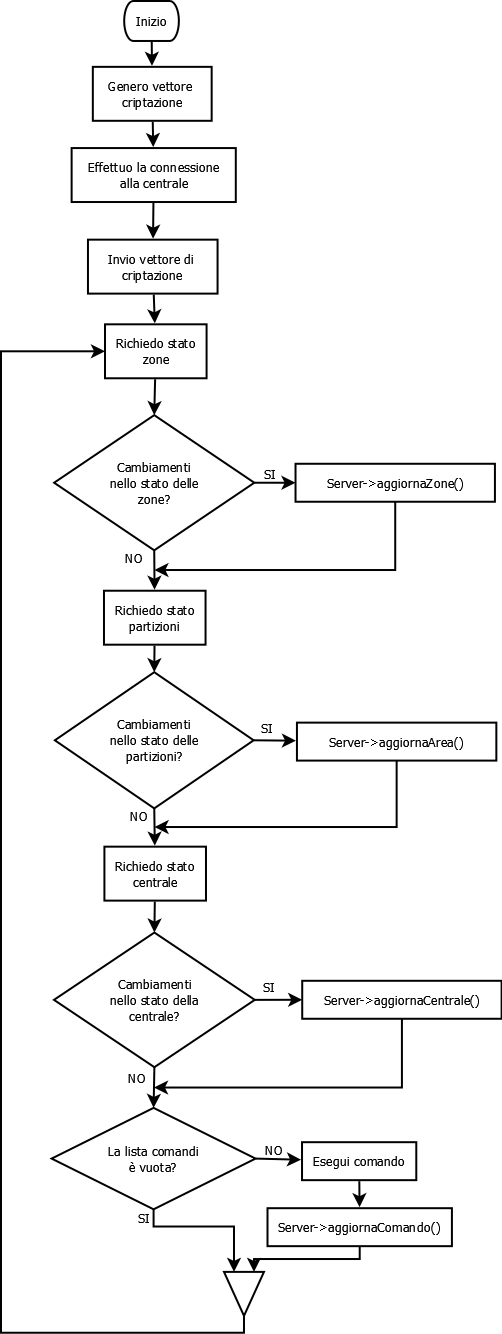
\includegraphics[width=0.7\linewidth]{pictures/runtecno.png}
	\caption{Diagramma di flusso del metodo Run della classe Tecnoalarm}\label{fig:flussotecno}
\end{figure}
\begin{lstlisting}[language=C++,caption=Costruttore della classe Tecnoalarm,label=lst:costtecno]
TecnoAlarm (long codice, Server* server);
\end{lstlisting}
Gli altri metodi della classe non fanno altro che preparare i pacchetti da trasmettere. In particolare i metodi \texttt{criptaPaccetto} e \texttt{decriptaPacchetto} sfruttano la libreria \emph{openssl}\cite{openssl} per effettuare le operazioni di criptazione e decriptazione del pacchetto. Questi due metodi sono mostrati in \lname{lst:decripta} e \lname{lst:cripta}.
\begin{lstlisting}[language=C++,caption=Metodo decriptaPacchetto,label=lst:decripta]
int TecnoAlarm::decriptaPacchetto(unsigned char * pacchetto, int len) {
    unsigned char temp[512];
    memset(temp,0,512);
    AES_cfb128_encrypt(pacchetto,temp, len, &ekey, ivtemprx, &numdec, AES_DECRYPT);
    memcpy(pacchetto,temp,len);
    return 0; 
}
\end{lstlisting}
\begin{lstlisting}[language=C++,caption=Metodo criptaPacchetto,label=lst:cripta]
int TecnoAlarm::criptaPacchetto(unsigned char * pacchetto, int len) {
    AES_cfb128_encrypt(pacchetto,pacchetto, len, &ekey, ivtemptx, &numenc, AES_ENCRYPT);
    return 0;
}
\end{lstlisting}
\subsubsection{Urmet}
Questa classe come detto eredita dalla classe \texttt{Centrale}. Il metodo \texttt{Run} si occupa solo di inviare la richiesta degli stati ed interpretare la risposta, una volta interpretata la confronta con gli stati precedenti e in caso di variazioni lo notifica al livello superiore. In \fname{fig:flussourmet} è mostrata la sequenza delle operazioni svolte dal metodo \texttt{Run}.
\begin{figure}
	\centering
	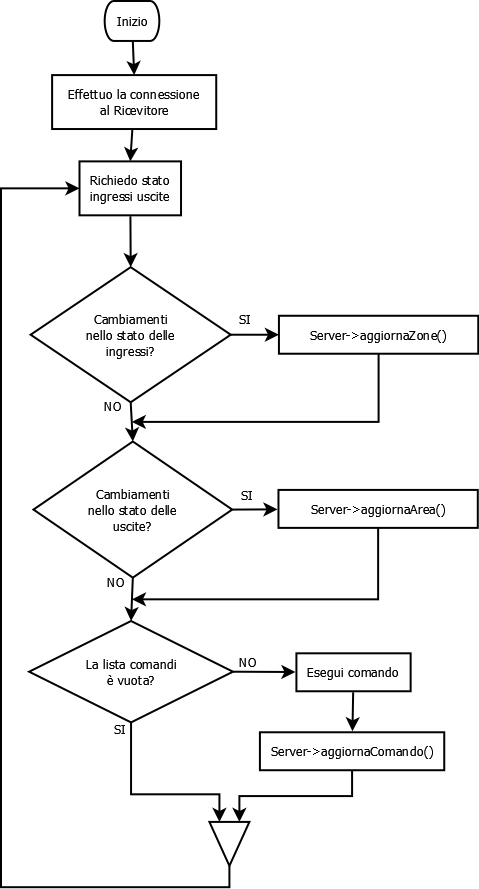
\includegraphics[width=0.7\linewidth]{pictures/teleurmet.png}
	\caption{Diagramma di flusso del metodo Run della classe Urmet}\label{fig:flussourmet}
\end{figure}
\subsubsection{Comandi}
Questa è la classica classe entità infatti essa rappresenta il generico comando, contiene due attributi che identificano il tipo di comando e l'elemento sul quale applicarlo.
\begin{lstlisting}[language=C++,caption=Classe Comandi, label=lst:comandi]
#ifndef COMANDI_H
#define COMANDI_H
enum enum_Comandi {
    ARM_PARTITION,
    DISARM_PARTITION,
    ARM_PARTIAL_PARTITION,
    INCLUDE_ZONE,
    EXCLUDE_ZONE,
    BLOCK_PROGRAM,
    UNBLOCK_PROGRAM };
class Comandi {
    public:
        Comandi (enum_Comandi comando, int elemento);
        virtual ~Comandi ();
        enum_Comandi getComando();
        int getElemento();
    private:
        enum_Comandi tipo_comando;
        int num_elemento;
};
\end{lstlisting}